
\section{Why Avi thinks block 3 is going to be problematic}

After the Cholesky parameterisation of the inverse spectral density,
\begin{equation}
S_k^{-1} = T_k^\dagger D_k^{-1} T_k ,
\end{equation}
the Whittle likelihood factorises into $p$ independent block likelihoods.
For block $j$, the resulting likelihood can be written as
\begin{equation}
\mathcal{L}_j \propto
\prod_{k=1}^N \delta_{jk}^{-2N_b}
\exp\!\left(
-\frac{1}{T\delta_{jk}^2}
\sum_{\omega=1}^{N_b}
\Bigl\|
u_{j\omega}^{(k)} - \sum_{l<j} \theta_{jl}^{(k)} u_{l\omega}^{(k)}
\Bigr\|^2
\right),
\end{equation}
where $\delta_{jk}^2$ is the diagonal scale parameter for block $j$.

Defining the frequency-wise residual power
\begin{equation}
R_{jk} \equiv
\sum_{\omega=1}^{N_b}
\Bigl\|
u_{j\omega}^{(k)} - \sum_{l<j} \theta_{jl}^{(k)} u_{l\omega}^{(k)}
\Bigr\|^2 ,
\end{equation}
and ignoring additive constants, the block log-likelihood becomes
\begin{equation}
\log \mathcal{L}_j
=
- N_b \sum_k \log \delta_{jk}^2
- \sum_k \frac{R_{jk}}{\delta_{jk}^2}.
\label{eq:block3_loglik}
\end{equation}

For block~$j=3$, we find that in some frequency bands the residual power is very small,
\begin{equation}
R_{3k} \approx 0 \quad \text{for many } k .
\end{equation}
In these regions the second term in Eq.~\eqref{eq:block3_loglik} has little effect, and the likelihood is dominated by
\begin{equation}
\log \mathcal{L}_3
\approx
- N_b \sum_k \log \delta_{3k}^2 .
\end{equation}
This expression increases without bound as $\delta_{3k}^2 \to 0$, so the likelihood prefers arbitrarily small values of $\delta_{3k}^2$ rather than a finite optimum.

As a result, the posterior concentrates near the lower boundary of $\delta_{3k}^2$, regardless of the values of the regression coefficients $\theta_{3l}$.
Unless the prior enforces a sufficiently strong lower bound on $\delta_{3k}^2$, the posterior will collapse toward zero variance.
This creates a sharply curved posterior geometry, leading to poor sampling efficiency and pathological behaviour for HMC methods.

\avi{I also tested emcee, things didnt work}





\section{Renates gibbs update for the last block}


\subsection{Background: Gaussian linear regression}

Consider the standard Gaussian linear regression model
\begin{equation}
\mathbf{Y} = \mathbf{X}\boldsymbol{\beta} + \boldsymbol{\epsilon},
\qquad
\boldsymbol{\epsilon} \sim \mathcal{N}(\mathbf{0}, \mathbf{D}),
\end{equation}
with a Gaussian prior on the regression coefficients,
\begin{equation}
\boldsymbol{\beta} \sim \mathcal{N}(\mathbf{0}, \mathbf{V}).
\end{equation}
The conditional posterior distribution of $\boldsymbol{\beta}$ is then
\begin{equation}
\boldsymbol{\beta} \mid \mathbf{Y}
\sim
\mathcal{N}(\mathbf{m}_{\mathrm{post}}, \boldsymbol{\Sigma}_{\mathrm{post}}),
\end{equation}
where
\begin{equation}
\boldsymbol{\Sigma}_{\mathrm{post}}
=
\left(
\mathbf{V}^{-1} + \mathbf{X}^{\top}\mathbf{D}^{-1}\mathbf{X}
\right)^{-1},
\qquad
\mathbf{m}_{\mathrm{post}}
=
\boldsymbol{\Sigma}_{\mathrm{post}}
\mathbf{X}^{\top}\mathbf{D}^{-1}\mathbf{Y}.
\end{equation}

\subsection{Complex conditional likelihood}

We now derive a likelihood of the above form by conditioning on all
parameters except the complex coefficient $Q(\Omega_{21})$.

Define
\begin{equation}
Q(\Omega_{21})
=
\begin{pmatrix}
\Re(\Omega_{21}) \\
\Im(\Omega_{21})
\end{pmatrix}.
\end{equation}

The likelihood contribution for block~2, viewed as a function of
$Q(\Omega_{21})$ with all other quantities fixed at their current sampled
values, is
\begin{equation}
\mathcal{L}_2
\propto
\prod_{k=1}^{N}
\exp\!\left\{
-\frac{1}{T S_{2k}^2}
\sum_{q=1}^{p}
\left|
Q(u_{2q}^{(k)}) - \hat{W}(u_{2q}^{(k)})
-
\bigl(
Q(\Omega_{21}) + i\,\Im(\Omega_{21})
\bigr)
\bigl(
\Re(u_{1q}^{(k)}) + i\,\Im(u_{1q}^{(k)})
\bigr)
\right|^2
\right\}.
\end{equation}

This expression is quadratic in $\Re(\Omega_{21})$ and $\Im(\Omega_{21})$.
Expanding the squared modulus and grouping terms yields a sum of weighted
squared residuals.

\subsection{Effective means and variances}

Define the inverse variances
\begin{equation}
\sigma_q^{(k)\,2}
=
\frac{1}{
\Re(u_{1q}^{(k)})^2
+
\Im(u_{1q}^{(k)})^2
},
\end{equation}
and the corresponding conditional means
\begin{equation}
\mu_q^{(k)}
=
\frac{
\Re(u_{2q}^{(k)}) \Re(u_{1q}^{(k)})
+
\Im(u_{2q}^{(k)}) \Im(u_{1q}^{(k)})
+
2\,\Re(u_{1q}^{(k)}) \Im(u_{1q}^{(k)}) \Im(u_{2q}^{(k)})
}{
\Re(u_{1q}^{(k)})^2
+
\Im(u_{1q}^{(k)})^2
}.
\end{equation}

With these definitions, the likelihood can be written as
\begin{equation}
\prod_{k=1}^{N}
\exp\!\left[
-\frac{1}{T S_{2k}^2}
\sum_{q=1}^{p}
\frac{
\left(
\Re(b_{2q}^{(k)}) - \mu_q^{(k)}
\right)^2
}{
\sigma_q^{(k)\,2}
}
\right].
\end{equation}

\subsection{Factorisation over frequencies}

Completing the square over $q$ for each frequency $k$ yields
\begin{equation}
\prod_{k=1}^{N}
\exp\!\left[
-\frac{1}{T S_{2k}^2}
\frac{
\left(
\Re(b_{2k}^{(k)})
-
\sum_{q=1}^{p}
\mu_q^{(k)} / \sigma_q^{(k)\,2}
\right)^2
}{
\sum_{q=1}^{p}
1 / \sigma_q^{(k)\,2}
}
\right].
\end{equation}

Define the effective response variable
\begin{equation}
y_k
=
\sum_{q=1}^{p}
\frac{\mu_q^{(k)\,2}}{\sigma_q^{(k)\,2}},
\end{equation}
and the diagonal covariance
\begin{equation}
\mathbf{D}
=
\operatorname{diag}(d_1,\ldots,d_N),
\qquad
d_k
=
T S_{2k}^2
\sum_{q=1}^{p}
\frac{1}{\sigma_q^{(k)\,2}} .
\end{equation}

\subsection{Gaussian regression form}

Identifying the real component with a linear model,
\begin{equation}
\Re(b_{2k})
=
\mathbf{X}\boldsymbol{\beta},
\end{equation}
we obtain
\begin{equation}
\mathbf{y}
\sim
\mathcal{N}
\!\left(
\mathbf{X}\boldsymbol{\beta},
\operatorname{diag}
\left(
T S_{2k}^2
\sum_{q=1}^{p}
\frac{1}{\sigma_q^{(k)\,2}}
\right)
\right).
\end{equation}

This recovers the Gaussian regression form required for Gibbs sampling
of $\boldsymbol{\beta}$ with conjugate updates.

\subsection{Design matrix and prior}

The design matrix is constructed from spline basis functions,
\begin{equation}
\mathbf{X}
=
\begin{pmatrix}
B_1(f_1) & \cdots & B_H(f_1) \\
\vdots  &        & \vdots  \\
B_1(f_N) & \cdots & B_H(f_N)
\end{pmatrix},
\qquad
\boldsymbol{\beta}
=
\begin{pmatrix}
\omega_1 \\
\vdots \\
\omega_M
\end{pmatrix},
\end{equation}
with prior covariance
\begin{equation}
\mathbf{V} = (\Phi^\top \Phi)^{-1}.
\end{equation}



\section{Generation of SCIRDv1 TDI--2 LISA Noise}
\label{subsec:lisa_noise_generation}

We generate synthetic LISA instrumental noise directly at the level of the 
second--generation time–delay interferometry (TDI--2) observables 
$\{X,Y,Z\}$ using the \emph{SciRDv1} mission noise specification.
This procedure follows the standard LISA noise model described in
\citet{Prince2002, Tinto2014, Nam2023} and is consistent with the 
transfer functions implemented in \texttt{LISAanalysisTools}.

\paragraph{Base noise sources.}
Two fundamental instrumental noise contributions are included:
the optical metrology system (OMS) displacement noise
$S^{m}_{\rm op}(f)$ and the test--mass acceleration noise $S^{a}_{\rm pm}(f)$.
For the SciRDv1 requirements these are parametrized as
%
\begin{align}
S^{m}_{\rm op}(f)
&=
A_{\rm OMS}^2
\left[
1 + \left(\frac{f_{\rm knee}}{f}\right)^4
\right],
\\[6pt]
S^{a}_{\rm pm}(f)
&=
A_{\rm TM}^2
\left[
1 + \left(\frac{f_{\rm low}}{f}\right)^2
\right]
\left[
1 + \left(\frac{f}{f_{\rm high}}\right)^4
\right],
\end{align}
%
where $A_{\rm OMS}$ and $A_{\rm TM}$ are the displacement and 
acceleration amplitude spectral densities respectively, and
$f_{\rm knee}$, $f_{\rm low}$, and $f_{\rm high}$ specify the low-
and high-frequency spectral turnovers.

Test-mass acceleration noise is first converted to displacement noise via
\begin{equation}
S^{m}_{\rm pm}(f)
=
\frac{S^{a}_{\rm pm}(f)}{(2\pi f)^4}.
\end{equation}

\paragraph{Conversion to frequency noise.}
Both displacement-noise contributions are converted to
\emph{absolute frequency noise} (units of $\mathrm{Hz}^2/\mathrm{Hz}$)
according to
%
\begin{equation}
S_{\Delta\nu}(f)
=
\left( \frac{2\pi f \nu_0}{c} \right)^2
S^{m}(f),
\end{equation}
%
where $\nu_0$ is the laser carrier frequency and $c$ is the speed of light.
This step produces frequency-noise PSDs
$S_{\rm op}(f)$ for the OMS contribution and
$S_{\rm pm}(f)$ for the test-mass contribution.

\paragraph{TDI--2 transfer functions.}
The frequency-noise PSDs are projected into the TDI--2 observables using
analytic transfer functions derived in \citet{Nam2023}.
Defining the dimensionless frequency variable

\begin{equation}
x \equiv 2\pi f \frac{L}{c},
\end{equation}

where $L$ is the LISA arm length, the diagonal and cross-channel
transfer factors for the Michelson $X$ channel take the form
%
\begin{align}
C_{XX}(f) &= 16 \sin^2 x \, \sin^2 (2x),
\\[4pt]
C_{XY}(f) &= -16 \sin x \, \sin^3 (2x).
\end{align}
%
By symmetry the $Y$ and $Z$ channels share identical diagonal forms,
and the cross-spectra $S_{YZ}$ and $S_{ZX}$ are equivalent to $S_{XY}$.

Using these transfer functions, the TDI-2 power spectral densities are
constructed as

\begin{align}
S_{XX}(f) &=
4\,C_{XX}(f)\,S_{\rm op}(f)
+
4\,C_{XX}(f)
\bigl[3+\cos(2x)\bigr]
S_{\rm pm}(f),
\\[6pt]
S_{XY}(f) &=
C_{XY}(f)\,S_{\rm op}(f)
+
4\,C_{XY}(f)\,S_{\rm pm}(f),
\end{align}
%
with analogous expressions for $S_{YY}$, $S_{ZZ}$ and the remaining
cross terms.  Together these define the full
$3\times3$ frequency-dependent noise covariance matrix

\begin{equation}
\boldsymbol{\Sigma}(f)
=
\begin{pmatrix}
S_{XX} & S_{XY} & S_{ZX}\\
S_{YX} & S_{YY} & S_{YZ}\\
S_{XZ} & S_{ZY} & S_{ZZ}
\end{pmatrix}.
\end{equation}

All PSDs are expressed in units of absolute frequency noise
($\mathrm{Hz}^2/\mathrm{Hz}$).

\paragraph{Time-series synthesis.}
Correlated time-domain TDI noise realizations
$\{X(t),Y(t),Z(t)\}$ are generated by sampling from a multivariate complex
Gaussian distribution in the Fourier domain.
For each discrete frequency bin $f_k$ the Fourier coefficients are drawn as

\begin{equation}
\tilde{\mathbf{n}}(f_k)
=
\mathbf{L}(f_k)\,\boldsymbol{\epsilon}(f_k),
\end{equation}
%
where $\boldsymbol{\epsilon}$ is a vector of independent unit-variance
complex Gaussian deviates and
$\mathbf{L}(f_k)$ is the Cholesky factor of the covariance

\begin{equation}
\mathrm{Cov}[\tilde{\mathbf{n}}(f_k)]
=
\frac{N}{2\Delta t}\,
\boldsymbol{\Sigma}(f_k),
\end{equation}

with $N$ the number of time samples and $\Delta t$ the sampling cadence.
Finally, inverse real FFTs are applied to the three channels to obtain the
correlated TDI noise time series.
Welch power-spectral estimates computed from these simulations
reproduce the analytic TDI noise PSDs by construction.


\section{Computational complexity.}

Let $N$ be the number of fine frequencies and $B$ the number of coarse elements ($B = N_\mathrm{low} + N_\mathrm{bins}$). 
Precomputing the bin statistics requires $O(Np^2)$ operations (a single pass over the DFTs). 
Each likelihood evaluation thereafter scales as the unbinned case but with $N$ replaced by $B$, i.e.
\begin{equation}
\mathcal{O}(Bp^2),
\end{equation}
for the quadratic forms, plus the cost of evaluating the spline fields, approximately $\mathcal{O}(BK)$ per parameter family (where $K$ is the number of basis functions). 
For typical settings $B \ll N$, runtime is reduced by roughly $N/B$ while preserving the same likelihood structure.


\section{Using Prior Knowledge of the LISA PSD and CSD}

Assume that we know the LISA design spectral density matrix $S_0(f)$, from instrument modelling.  
This matrix contains the expected auto-spectra (PSD) and cross-spectra (CSD) between channels, and its overall magnitude and structure are known to be physically reasonable.  
We describe two simple ways to incorporate this information into the multivariate P-spline model.

\subsection{Soft shrinkage toward the design spectrum}

The idea is to let the estimated spectrum $S(f)$ stay close to $S_0(f)$ unless the data provide strong evidence that the true spectrum differs.

Our model parameterises the inverse spectral matrix through the modified
Cholesky decomposition
$$\bold{S}(f_k)^{-1} = \bold{T}_k^* \bold{D}_k^{-1} \bold{T}_k$$
where $\bold{D}_k(f)$ contains the innovation variances and $\bold{T}_k(f)$ contains the (off-diagonal) regression terms.  
Both are represented as smooth P-spline functions.

We compute the same decomposition for the known design spectrum,
$$\bold{S}_0(f_k)^{-1} = \bold{T}_{0,k}^* \bold{D}_{0,k}^{-1} \bold{T}_{0,k}$$
and then place simple Gaussian priors on the spline coefficients, centred at the design values.  
For example,
$$\text{spline coefficients of }\log\delta_j^2(f)
   \sim \mathcal{N}\bigl(\text{design coefficients},\; \tau_{\delta,j}^2\bigr),$$
and similarly for the off-diagonal terms $\theta_{jl}(f)$.
Small values of $\tau$ keep the inferred PSD/CSD near the LISA design curve.
Larger values let the data pull the estimate away more freely.  
\color{teal}
Could this be an easy and statistically safe way to ``regularise'' the fit using the known physics of the instrument?
\color{black}

For demonstration, look at figure~\ref{fig:shrinkage}.


\begin{figure}
    \centering
    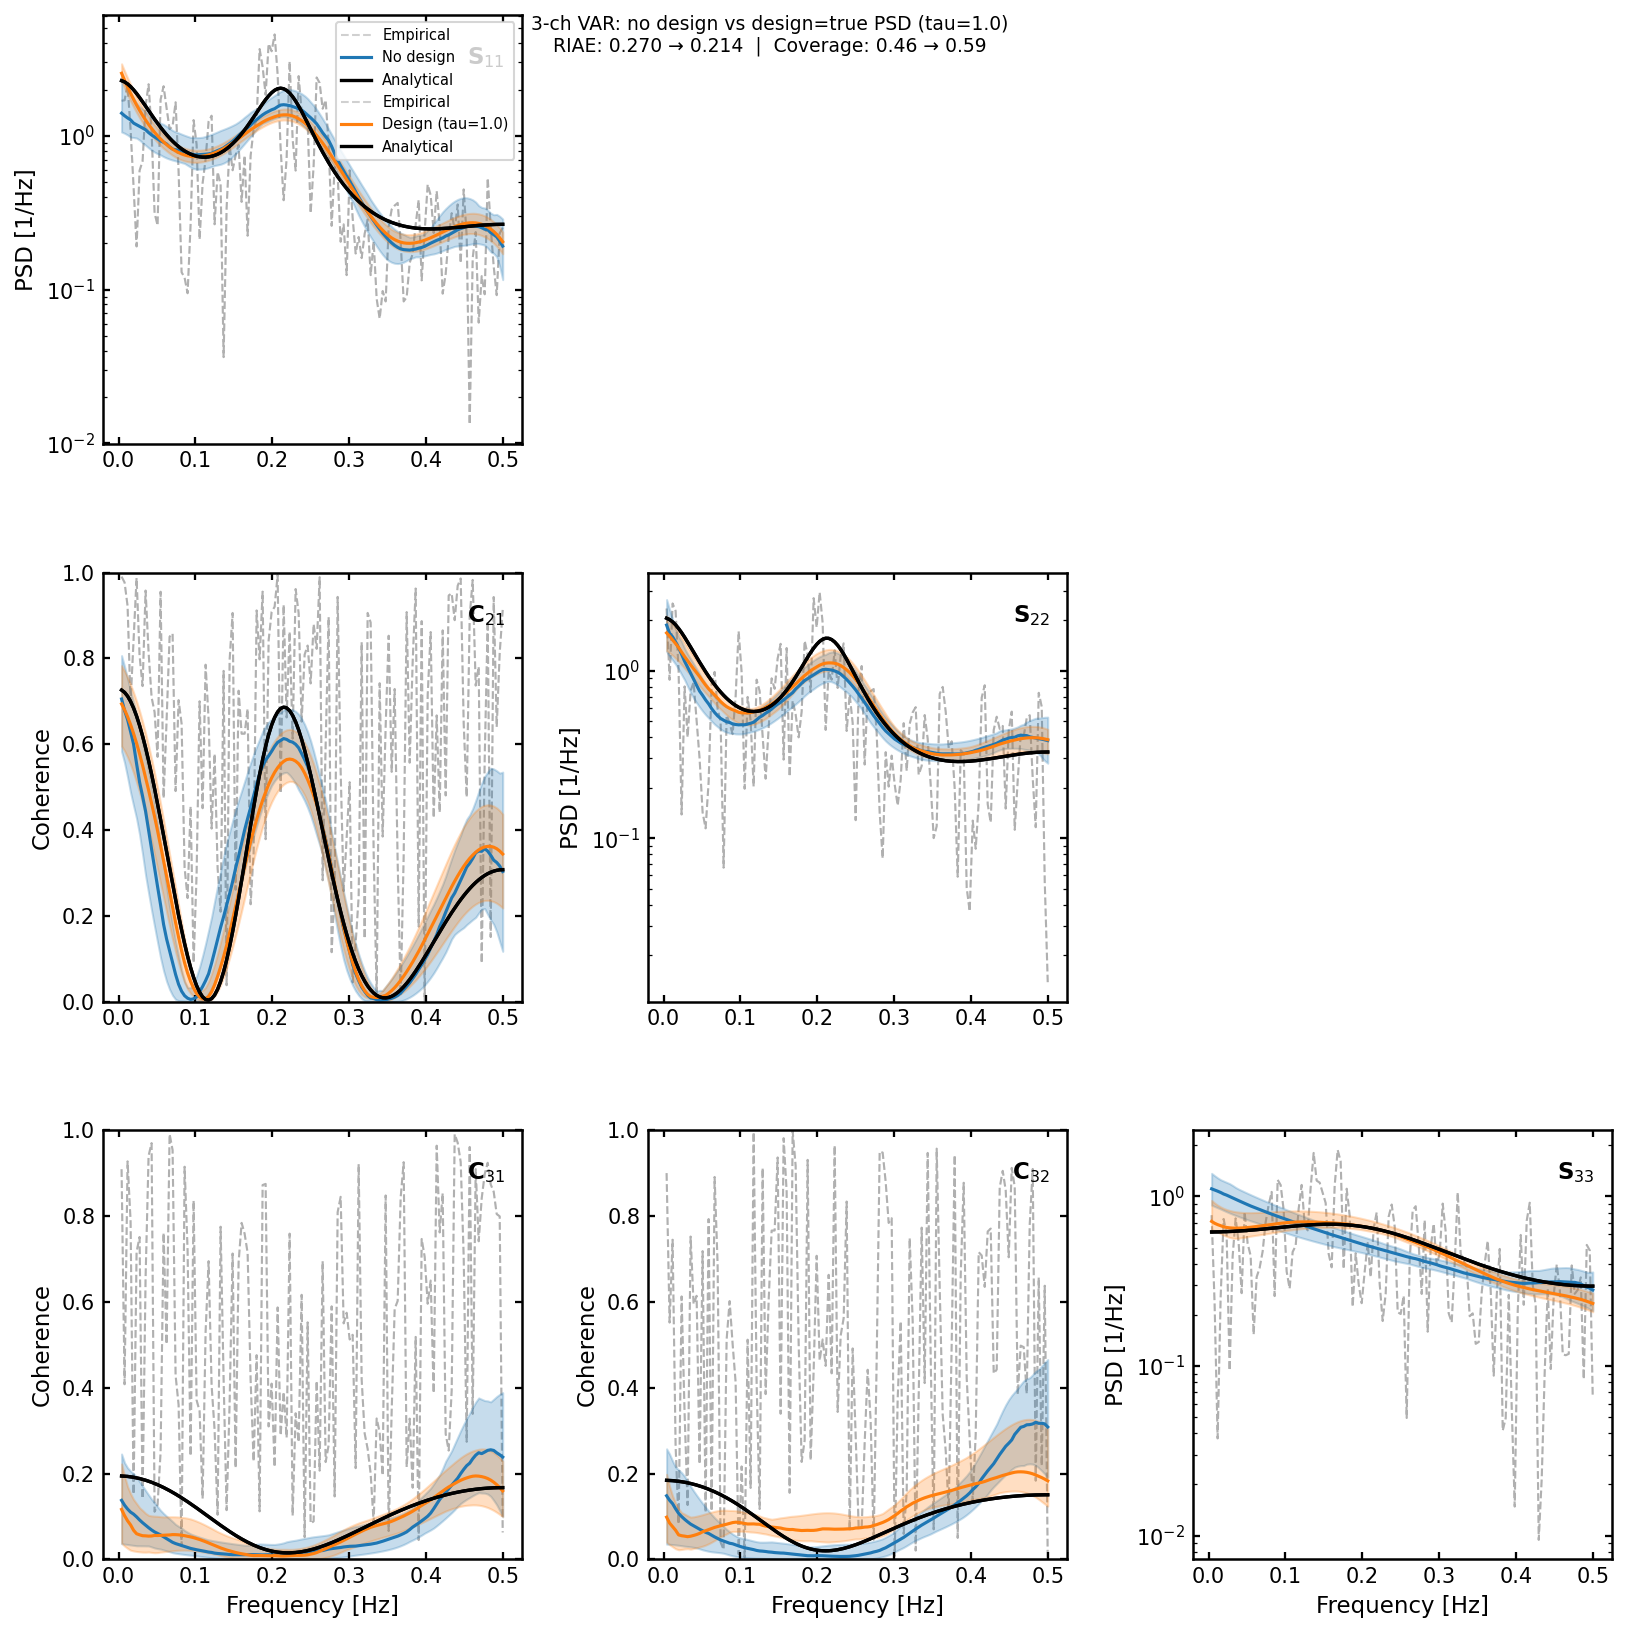
\includegraphics[width=0.95\linewidth]{figures/design_vs_no_design_comparison.png}
    \caption{Example of shrinkage in action}
    \label{fig:shrinkage}
\end{figure}


\subsection{Hard upper/lower bounds on PSD and CSD}

If we have physical bounds on the spectrum--for instance, known minimum/maximum levels that each auto-spectrum $S_{jj}(f)$ must lie within—these constraints can be imposed directly in the model.


To guarantee that the estimated PSD stays within physically allowed
limits, for example
$$ L_j(f) \le S_{jj}(f) \le U_j(f),$$
we replace the usual unconstrained spline model with a bounded reparameterisation.  
Let $z_j(f)$ be any smooth spline function (with no constraints).  
Although $z_j(f)$ is written as a spline expansion,
$$
  z_j(f) = \sum_k B_k(f)\, w_{jk},
$$
it is \emph{not} the log-PSD.  
It is only an unconstrained latent variable.  
The PSD is then constructed by mapping $z_j(f)$ into the allowed interval $[L_j(f), U_j(f)]$ using the logistic transform, $\sigma(x)=1/(1+e^{-x})$:
$$
  \log S_{jj}(f)
    = \log L_j(f)
      + \sigma\!\big(z_j(f)\big)\,
        \big[\log U_j(f)-\log L_j(f)\big].
$$
Because $\sigma(z)\in(0,1)$ for all real $z$, the resulting PSD automatically satisfies the required bounds at every frequency, independently of the spline coefficients.  
This allows prior knowledge of the physically allowed PSD range to be imposed in a simple and stable way.

For the diagonal elements (PSD), one can restrict $\delta_j^2(f)$ to lie between frequency-dependent limits $a_j(f)$ and
$b_j(f)$ derived from the LISA design model:
$$  a_j(f) \le \delta_j^2(f) \le b_j(f).$$
This can be done by reparameterising the spline representation using a logistic transform, which automatically keeps the values inside the allowed band.


\avi{Ask renate and patrico for help for the cross spectra...}
For the cross-spectra it might be more convenient to work with the complex coherence,
$$
  C_{lm}(f)
    = \frac{S_{lm}(f)}
           {\sqrt{S_{ll}(f)\,S_{mm}(f)}},
\qquad
  |C_{lm}(f)| \le 1.
$$
Modelling the CSD directly can violate this constraint and can lead to
a non–positive-semidefinite spectral matrix.  Instead, we parameterise
$C_{lm}(f)$ in polar form,
$$
  C_{lm}(f) = \tanh(r_{lm}(f))\,e^{i\phi_{lm}(f)},
$$
where $r_{lm}(f)$ and $\phi_{lm}(f)$ are unconstrained spline functions.  
Since $\tanh(r)\in(-1,1)$ for all real $r$, this representation automatically enforces $|C_{lm}(f)|<1$ at every frequency. 
The corresponding cross-spectrum is then constructed as
$$
  S_{lm}(f)
    = C_{lm}(f)\,\sqrt{S_{ll}(f)\,S_{mm}(f)}.
$$
If the LISA design model provides a prior coherence curve $C_{0,lm}(f)$, we decompose it into magnitude and phase and place Gaussian priors on the spline coefficients of $r_{lm}(f)$ and $\phi_{lm}(f)$ centred at the design values.  
This keeps the inferred coherence close to the physically motivated LISA model while allowing the data to make adjustments.



\section{Blocked updates for the third Cholesky component}

For $p=3$, the third likelihood factor is
\begin{align}
\mathcal{L}_3
&\propto
\prod_{k=1}^{N}
(\delta_{3k}^2)^{-N_b}
\exp\!\left(
-\frac{1}{T\delta_{3k}^2}
\sum_{\nu=1}^{p}
\left|
u^{(k)}_{3\nu}
-
\theta_{31}^{(k)} u^{(k)}_{1\nu}
-
\theta_{32}^{(k)} u^{(k)}_{2\nu}
\right|^2
\right).
\end{align}

\subsection{Conditional update for $\theta_{31}$}

Fix $\theta_{32}^{(k)}$ and define partial residuals
\[
\tilde r^{(k)}_{\nu}
=
u^{(k)}_{3\nu}
-
\theta_{32}^{(k)} u^{(k)}_{2\nu}.
\]
Then
\[
\sum_{\nu}
\left|
\tilde r^{(k)}_{\nu}
-
\theta_{31}^{(k)} u^{(k)}_{1\nu}
\right|^2
=
a_k |\theta_{31}^{(k)}|^2
-
2\Re\!\left(\theta_{31}^{(k)} b_k\right)
+ \text{const},
\]
where
\[
a_k = \sum_{\nu} |u^{(k)}_{1\nu}|^2,
\qquad
b_k = \sum_{\nu} u^{(k)*}_{1\nu}\tilde r^{(k)}_{\nu}.
\]

Let $\theta_{31}^{(k)} = B_{k\cdot} w_{31}$ be a spline expansion with basis matrix $B$.
Define
\[
W_k = \frac{a_k}{T\delta_{3k}^2},
\qquad
c_k = \frac{b_k}{T\delta_{3k}^2}.
\]
Then the conditional likelihood is quadratic in $w_{31}$:
\[
\log p(\text{data}\mid w_{31},\cdot)
=
- w_{31}^* Q_{\text{like}} w_{31}
+
2\Re\!\left(w_{31}^* \ell_{\text{like}}\right)
+ \text{const},
\]
with
\[
Q_{\text{like}} = B^\top W B,
\qquad
\ell_{\text{like}} = B^\top c.
\]

With the Gaussian P-spline prior
\[
w_{31} \mid \phi_{31} \sim \mathcal{N}\!\left(0,(\phi_{31} P_{31})^{-1}\right),
\]
the conditional posterior is
\[
w_{31} \mid \cdot
\sim
\mathcal{N}\!\left(
Q_{\text{post}}^{-1}\ell_{\text{like}},
\; Q_{\text{post}}^{-1}
\right),
\qquad
Q_{\text{post}} = \phi_{31} P_{31} + Q_{\text{like}}.
\]

Real and imaginary spline weights are updated independently using the same precision matrix $Q_{\text{post}}$.

\newpage

\subsection{Conditional update for $\theta_{32}$}



Fix $\theta_{31}$ and define
\[
\bar r^{(k)}_{\nu}
=
u^{(k)}_{3\nu}
-
\theta_{31}^{(k)} u^{(k)}_{1\nu}.
\]
Repeating the above steps yields a Gaussian conditional posterior for the spline weights
$w_{32}$ with precision
\[
Q^{(32)}_{\text{post}} = \phi_{32} P_{32} + B^\top W' B,
\]
where
\[
W'_k = \frac{\sum_\nu |u^{(k)}_{2\nu}|^2}{T\delta_{3k}^2}.
\]

\subsection{NUTS update for $\delta_3$}

The remaining parameters are the spline weights $w^{(\delta)}_3$ defining
\[
\log \delta_{3k}^2 = B^{(\delta)}_{k\cdot} w^{(\delta)}_3.
\]
Their conditional posterior is non-Gaussian due to the terms
$\log \delta_{3k}^2$ and $1/\delta_{3k}^2$ in the likelihood, so $w^{(\delta)}_3$
is updated using NUTS conditional on $\theta_{31},\theta_{32}$.

\subsection{One full iteration}

One sampler iteration consists of:
\begin{enumerate}
\item Draw $w_{31}$ from its Gaussian conditional.
\item Draw $w_{32}$ from its Gaussian conditional.
\item Run NUTS targeting $p(w^{(\delta)}_3 \mid w_{31}, w_{32}, \text{data})$.
\end{enumerate}
